\chapter{Análise Bibliográfica sobre Mineração de Dados Educacionais, por Pedro de Torres Maschio\label{chap:bibliometria:pedro-maschio}}


\section{Planejamento do estudo}

O crescente uso de plataformas de aprendizagem remota, conhecidos como Ambientes Virtuais de Aprendizagem (AVAs) aumentou consideravelmente a produção de dados sobre como os alunos aprendem e sobre como usam estas plataformas. Essa crescente quantidade de informação deu origem a um tipo de mineração de dados específica, a Mineração de Dados Educacionais. O presente estudo busca evidenciar aspectos a respeito da produção científica sobre esse tema. As questões de pesquisa são:

\begin{itemize}
    \item Como a produção científica em Mineração de Dados Educacionais evoluiu ao longo do tempo?
    \item Quais são os principais conceitos relacionados a Mineração de Dados Educacionais?
    \item Como a Mineração de Dados Educacionais tem sido utilizada para subsidiar ações práticas de ensino remoto?
\end{itemize}

\section{Coleta de dados}

A coleta de dados se deu pelo Web of Science (WeS) no dia 6 de Fevereiro de 2022. O acesso foi feito por meio do Periódicos Capes. A base que foi utilizada para a busca foi "Science Citation Index Expanded", que reúne artigos da área de ciências exatas. A \textit{string} de busca pode ser vista na listagem de código \ref{pedro-maschio:listagem}

\lstinputlisting[numbers=left,basicstyle=\normalsize\ttfamily,caption={\query\ de busca sobre Mineração de Dados Educacionais.},label=pedro-maschio:listagem]
{experiments/pedro-maschio/PesquisaBibliogr/queries/query.txt}


Inicialmente, havia sido utilizado apenas o termo "educacional data mining", após uma análise dos resultados, observou-se que uma considerável parte dos resultados tratavam-se de revisões de literatura sobre o tema, sendo assim, adicionou-se a cláusula "not review" à \textit{string} de busca.
O uso desse termo de busca resultou em 5.156 resultados na WeS. A exportação desses registros foi feita com o uso da opção "Exportar arquivo de texto sem formatação", o conteúdo foi definido com a seleção personalizada de todos os 29 campos disponíveis para marcação. Os registros foram extraídos de mil em mil e depois concatenados no único arquivo de texto de forma manual.

\subsection{Filtragem dos dados}

Após a coleta, foram considerados somente registros de artigos científicos publicados em períodicos. Sendo assim, restaram 4.700 registros para análise. De agora em diante esse conjunto de registros será chamado EDM@pedro-maschio.

\section{Análise dos dados}

\subsection{Análise descritiva}

O bibliometrix, por meio da interface biblioshiny permite extrair uma tabela contendo as principais informações sobre os artigos contidos no EDM@pedro-maschio, abaixo estão listadas algumas dessas informações:
\begin{description}
    \item[Timespan] os artigos do \textit{dataset} EDM@pedro-maschio abrangem os anos de 1991 a 2022, o que ressalta o quão novo é o campo de estudo em Mineração de Dados Educacionais, tendo em vista que não foram encontrados artigos entre 1945 e 1990.
    \item[Sources (Journals, Books, etc)] há 1445 fontes de informação no \textit{dataset} EDM@pedro-maschio.
    \item[Documents] há 4700 documentos no \textit{dataset} EDM@pedro-maschio, sendo todos artigos científicos.
    \item[Average years from publication] a média de anos de publicação do \textit{dataset} EDM@pedro-maschio é de 4.46.
    \item[Average citations per documents] a média de citações por documento é de 14.4 no \textit{dataset} EDM@pedro-maschio.
    \item[Average citations per year per doc] a média de citações por ano por documento é de 2.349 no \textit{dataset} EDM@pedro-maschio.
    \item[References] há 169101 referências no \textit{dataset} EDM@pedro-maschio.
    \item[Keywords Plus (ID)] há 9501 Keywords Plus (ID) no \textit{dataset} EDM@pedro-maschio.
    \item[Author's Keywords (DE)] há 14652 palavras-chave que foram adicionadas pelos autores no \textit{dataset} EDM@pedro-maschio.
    \item[Authors] há 14911 nomes de autores distintos no \textit{dataset} EDM@pedro-maschio
    \item[Author Appearances] os 14911 autores distintos aparecem 28196 no \textit{dataset} EDM@pedro-maschio.
    \item[Authors of single-authored documents] 111 autoes publicaram artigos sem co-autores no \textit{dataset} EDM@pedro-maschio.
    \item[Authors of multi-authored documents] 14800 autores foram autores de artigos em conjunto com outros autores no \textit{dataset} EDM@pedro-maschio.
    \item[Single-authored documents] 128 artigos foram escritos por um único autor no \textit{dataset} EDM@pedro-maschio.
    \item[Documents per Author] a taxa de documentos por autor é de 0.315 no \textit{dataset} EDM@pedro-maschio.
    \item[Authors per Document] a taxa de autor por documento é de 3.17 no \textit{dataset} EDM@pedro-maschio.
    \item[Co-Authors per Documents] há em média 6 autores por artigos no \textit{dataset} EDM@pedro-maschio.
    \item[Collaboration Index] o índice de colaboração é de 3,24 no \textit{dataset} EDM@pedro-maschio.
\end{description}

\section{Visualização dos dados}

\subsection{Evolução da produção Científica}

\begin{figure}[H]
    \centering
    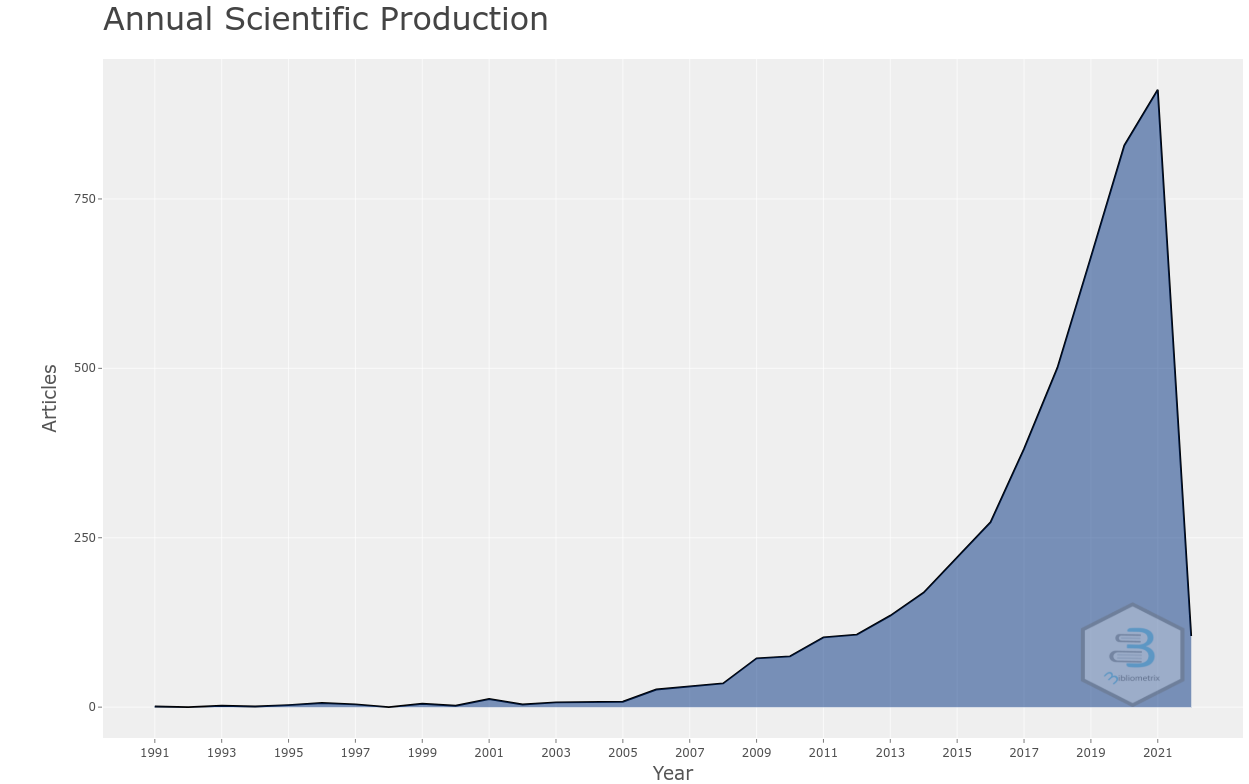
\includegraphics[width=1\textwidth]{experiments/pedro-maschio/PesquisaBibliogr/MineracaoDadosEducacionais/images/crescimento-anual.png}
    \caption{Evolução da produção científica no \textit{dataset} EDM@pedro-maschio.}
    \label{fig:evol:anual:EDM@pedro-maschio}
\end{figure}

Conforme apresenta-se na Figura \ref{fig:evol:anual:EDM@pedro-maschio}, a produção de artigos referente à Mineração de Dados Educacionais cresceu vertiginosamente, tendo seu início de fato a partir do ano 2005. A taxa média de crescimento anual foi de 17.41\%. 

\subsection{Citações média por ano}

\begin{figure}[H]
    \centering
    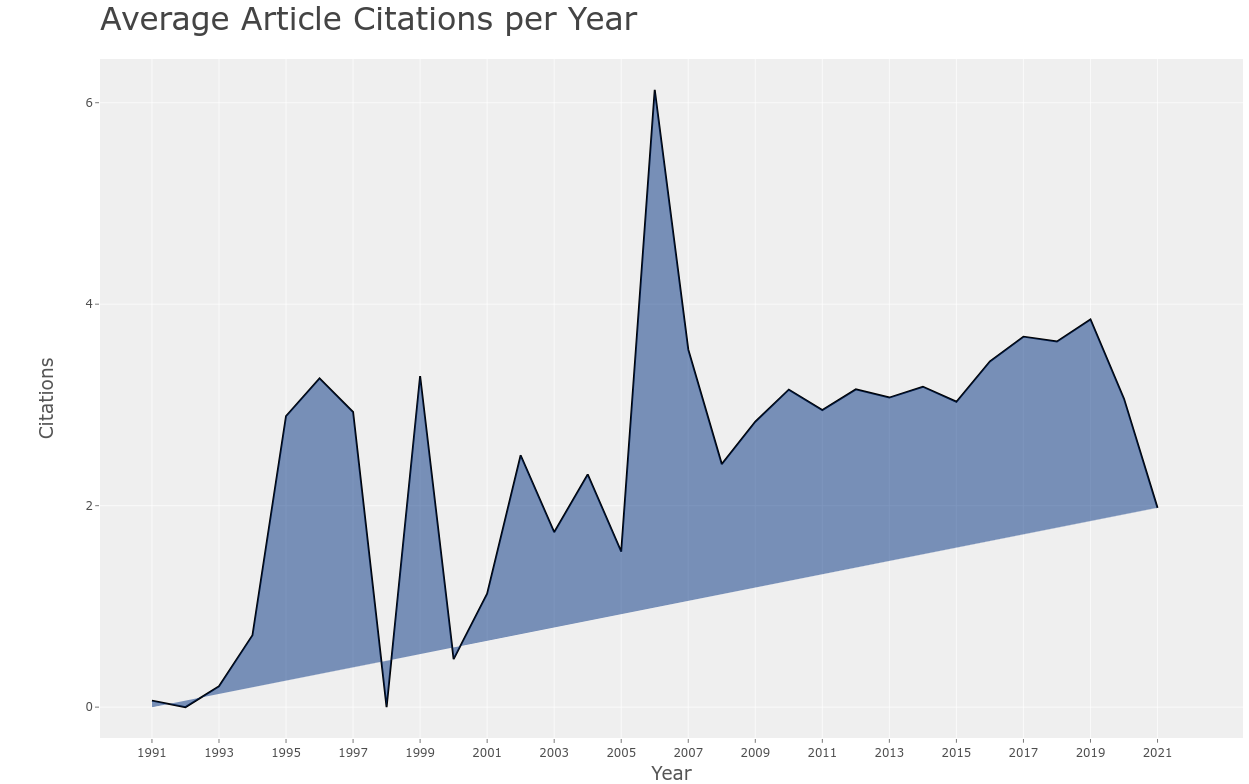
\includegraphics[width=1\textwidth]{experiments/pedro-maschio/PesquisaBibliogr/MineracaoDadosEducacionais/images/citacoes-media-anual.png}
    \caption{Evolução da produção científica no \textit{dataset} EDM@pedro-maschio.}
    \label{fig:citacoes:anual:EDM@pedro-maschio}
\end{figure}

Além da evolução no número de artigos publicados por ano, é possível extrair a evolução do número de citações média por ano, conforme apresenta-se na Figura \ref{fig:citacoes:anual:EDM@pedro-maschio}. Interessante notar os picos nos anos 1996, 1999 e 2006.


\subsection{Conceitos relacionados}

A análise da estrutura conceitual do documento começou pela geração do gráfico da Rede de Co-Ocorrências de Palavras-Chave. Este gráfico está evidenciado na Figura \ref{fig:co-ocorrencias:EDM@pedro-maschio}. Pela análise do gráfico gerado é possível observar a prevalência dos termos \textbf{modelo, predição, classificação, algoritmo e performance}; tais termos estão condizentes com o tema de Mineração de Dados Educacionais e dão \textit{insights} dos conceitos relacionados a essa área.

\begin{figure}[H]
    \centering
    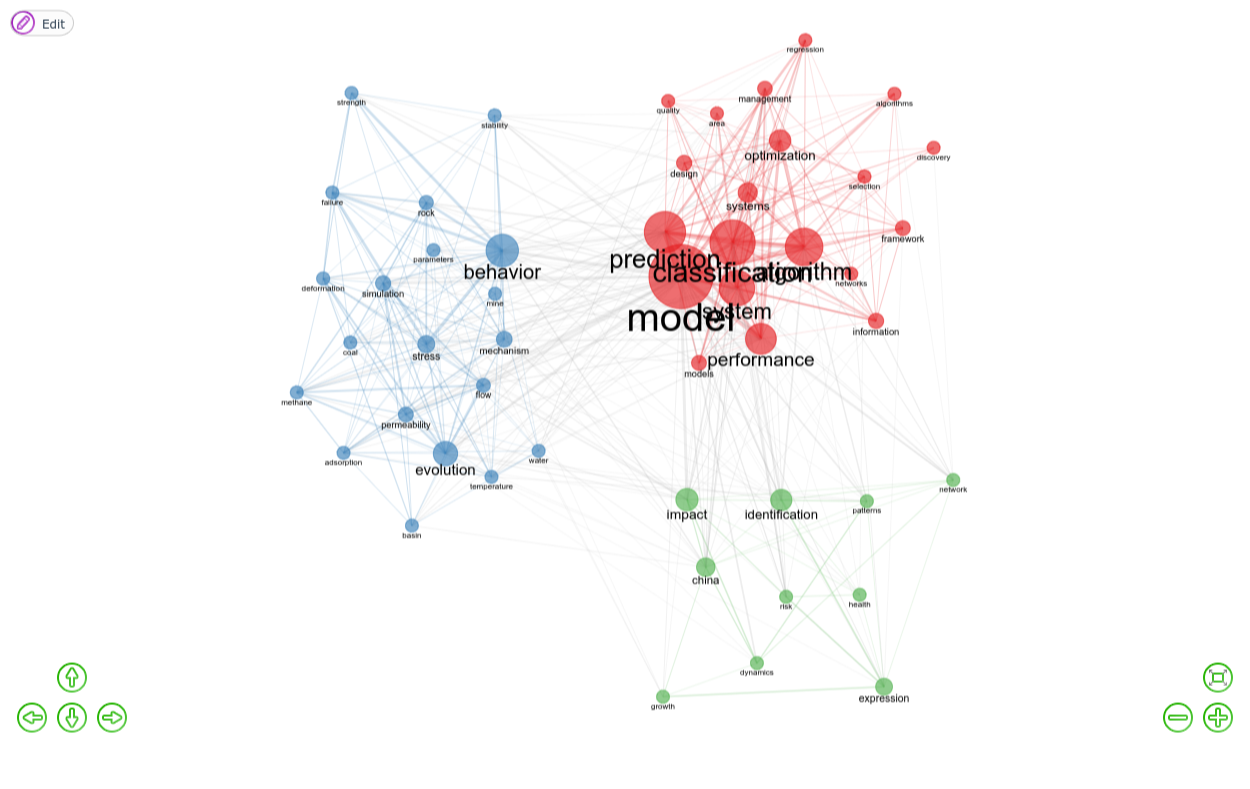
\includegraphics[width=1\textwidth]{experiments/pedro-maschio/PesquisaBibliogr/MineracaoDadosEducacionais/images/co-ocorrencias.png}
    \caption{Rede de co-ocorrências de palavras chave do \textit{dataset} EDM@pedro-maschio.}
    \label{fig:co-ocorrencias:EDM@pedro-maschio}
\end{figure}


\section{Resultados e interpretação}

Esta pesquisa bibliográfica indicou um crescente apelo da comunidade científica por buscas no campo de Mineração de Dados Educacionais. Os picos apresentados no gráfico de citações precisam ser melhor compreendidos por meio de uma busca mais aprofundada.
